\chapter{Formazione del segnale}

Tipicamente i detector sfruttano le cariche generate dalle particelle che ionizzano la materia e sfruttano campi elettrici e magnetici per spostarle.
\\
Nel detector possiamo distinguere 2 tipi di movimenti:
\begin{itemize}
    \item \textbf{Disordinati}: con una distribuzione di velocità (Maxwell-Boltzmann nel limite classico. Nei semi conduttori può diventare importante l'effetto quantistico) data dall'energia termica che causa una dispersione della carica. Il campo elettrico può cambiare questa distribuzione
    \item \textbf{Moto di drift}: causato dalla presenza di campi elettrici e magnetici
\end{itemize}
La \textbf{velocità di drift} è data dall'equilibri dell'accelerazione della carica e le collisioni con gli altri atomi.
Solitamente $|v_d|\ll \left<v\right>$ dove $\left<v\right>$ è la media della velocità termica

\section{Equazione del trasporto}
L'\textbf{equazione di boltzmann} descrive l'evoluzione di posizione e velocità di una carica in un mezzo in funzione delle forze esterne. 
\\ 
\\ 
Consideriamo una nuvola di cariche in un mezzo con una distribuzione nello spazio delle fasi f (dp è un elemento infinitesimo dello spazio delle fasi)

\begin{figure}[H]
    \centering
    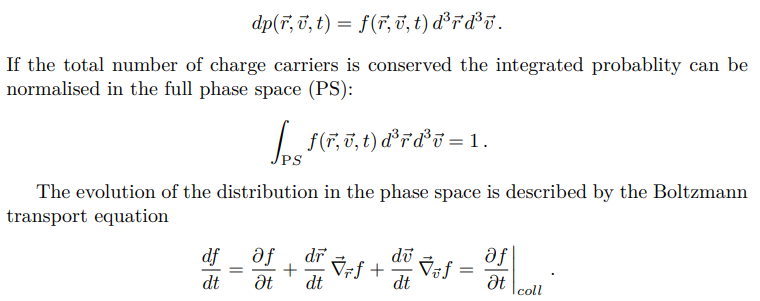
\includegraphics[width=0.8\textwidth,frame]{Chapters/images/Interazione_radiazione_materia/image-20220222095029391.png}
    \captionsetup{width=0.8\linewidth}
    \caption{Equazione del trasporto di Boltzmann}
    \label{fig:boltzmann}
\end{figure}
\begin{remark}[Commenti]
\hfill
\begin{itemize}
    \item $\partial_t f=0$ nel caso non ci sia dipendenza esplicita della densità dello sp. delle fasi dal tempo. 
  Quindi \textit{è nullo nel caso stazionario}

\item 2° termine descrive evoluzione nella posizione (diffusione)

\item 3° termine descrive evoluzione nella velocità

\item $\partial_tf|_\text{coll}$ è detto integrale di collisione (infatti eq. Boltzmann è un'equazione integro-differenziale). In questo termine entrano tutte le possibili sezioni d'urto a cui le cariche sono soggette
\end{itemize}


\end{remark}

\begin{note}[Integrale di collisione]
    \[\at{\frac{\partial f}{\partial t}}{coll}{}=\int W(\vec{v}_1,\vec{v} _{2} ;\vec{v} _{3}, \vec{v}) \{ f(\vec{r} ,\vec{v} _{1} ,t)f(\vec{r} , \vec{v} _{2} t)-f(\vec{r} ,\vec{v} _{3},t) f(\vec{r} ,\vec{v} ,t)\} d \vec{v} _{1} d \vec{v} _{2} d \vec{v} _{3}   \]


\begin{figure}[H]
    \centering
    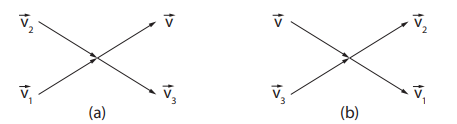
\includegraphics[width=0.8\textwidth,frame]{Chapters/images/Interazione_radiazione_materia/image-20220222100641937.png}
\end{figure}
    \hspace{-15pt}
    \begin{minipage}{0.48\textwidth}
        \begin{figure}[H]
            \centering

            \captionsetup{width=\textwidth}
            \caption{\\
            A: Il termine positivo è dato dall'aumento di densità causato all'aumento della velocità a causa di una collisione entrante che fa accelerare la particella \\
            B: Il termine negativo rappresenta una  diminuzione della densità causata dalla collisione della particella con altri atomi che ne causa una perdità di energia}
            \label{fig:}
        \end{figure}
    \end{minipage} \hspace{20pt}
    \begin{minipage}{0.4\textwidth}
    
        Integrale di collisione nel caso di scattering elastico $1+2\to3+4$.\\
         E' la probabilità che la particella 1 e 2 che si incontrano al tempo t nel punto r scatterino in una seconda coppia con velocità v e $v_3$ e viceversa (W è simmetrica per scambio delle coppie)
    
    \end{minipage}
\end{note}

\subsubsection*{Approssimazioni}
Alcune approssimazioni utili che rendono l'equazione analiticamente risolvibile sono:
\begin{itemize}
    \item \textbf{Equilibrio (Maxwell-boltzmann)}: Caso in cui non ci sono forze e f(r,v,t)=f(v). In questo caso l'integrale di collisione è nullo.

$$
f_0(\vec{v})=C \exp(-Av^2)
$$

\item \textbf{Approssimazione di rilassamento}: Assumiamo che dopo un'interazione il sistema impieghi un \textit{tempo di rilassamento} $\tau$ per tornare all'equilibrio. 
  Sotto questa assunzione vale $\partial_tf|_\text{collision}=-\frac{f-f_0}{\tau}$ dove $f_0$ è la soluzione nel caso di equilibtio. 
  La soluzione sarà:
  $$
  f(t)=f_0+(f-f_0)e^{-\frac{t}{\tau}}
  $$
  Questa approssimazione è \textit{molto utile nei detector} che sono sistemi in qui l'equilibrio è ripristinato dopo un tempo caratteristico

  \item \textbf{Campo elettrico costante}: In questa approssimazione possiamo considerare la presenza di un campo elettrico costante: 
    \begin{itemize}
        \item Il 1° termine è nullo, stabilità implica indipendenza temporale

    \item Il 2° termine è nullo
    \item Il 3° termine è dato da $\frac{dv}{dt}=\frac{qE}{m}$
    \end{itemize}
    

    Un'altra approssimazione che si può fare è $\nabla_v f \sim \nabla_vf_0$

    Se esprimiamo tutto in funzione dell'energia cinetica T otteniamo
    $$
    f= f_0-eQ\tau v_3\partial_Tf_0
    $$
    Ovviamoente la distribuzione è anisotropa e preferisce la direzione del campo E

\end{itemize}

\subsection{Velocità di Drift}
La \textbf{velocità di drift} è la velocità media (vettoriale) delle cariche
$$
\vec{v_D}=\int \vec{v} f(\vec{v})d^3\vec{v}
$$
Questa velocità è non nulla solo se f presenta una asimmetria nello spazio degli impulsi.
Conviene rappresentare questa asimmetria in termini di distribuzioni angolari e quindi esprimendo le velocità in coordinate sferiche.
\\ 
Esprimendo l'integrale in funzione dell'energia cinetica otteniamo 
\[
\begin{gathered}
        \vec{v_d}=\frac{2qE}{3m}<\tau>=\mu E
    \\ 
    \text{Mobilità: }\mu=\frac{2q}{3m} \left<\tau \right>\; :
    \\ 
    \text{Cammino libero medio: }\lambda=\tau v=\frac{1}{n\sigma}  
\end{gathered}  
\]
\begin{remark}[Misture]\hfill \\ 
    Per le misture vale $\frac{1}{\mu}=\sum_i \frac{f_i}{\mu_i}$ dove $f_i$ sono le abbondanze. 
Questa legge vacilla quando iniziano a esserci importanti scambi di carica tra gli ioni e le molecole del gas con diversa mobilità
\end{remark}
Il tempo medio $\tau$ che intercorre tra 2 successive collisioni è dato dalle sezioni d'urto in gioco ed è esprimile in funzione del cammino libero medio.

\begin{note}
    $\tau$ non è il tempo di rilassamento come definito prima ma è il tempo di collision. Ad ogni collisione le velocità sono in media distribuite isotropicamente e l'energia guadagnata dalla particella è dispersa, quindi il sistema torna all'equilibrio
\end{note}
La mobilità è fortemente dipendente dal campo E in quanto lo sono anche tutte le sezioni d'urto coinvolte nelle collisioni. Questo causa fenomeni di saturazione (o addirittura di diminuzione nei gas) della velocità di drift per campi elettrici molto alti.

\begin{remark}[Presenza di campo magnetico]
    \hfill
    \\
    \hspace{-20pt}
\begin{minipage}{0.48\textwidth}
    \begin{figure}[H]
        \centering
        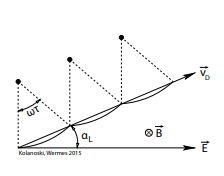
\includegraphics[width=\textwidth,frame]{Chapters/images/Interazione_radiazione_materia/image-20220222150553652.png}
        \captionsetup{width=\textwidth}
        \caption{Angolo di Lorentz}
        \label{fig:lorentzangle}
    \end{figure}
\end{minipage} \hspace{10pt}
\begin{minipage}{0.48\textwidth}
    Nel caso sia presente anche un campo B non si hanno cambiamenti nella velocità di drift e si ha una riduzione della diffusione: le cariche percorrono archi di curve.\\ 
    \\
    L'angolo formato dalla traccia con il campo elettrico sarà $\tan(\alpha_L)=\frac{v^B_x}{v^E_z}=w\tau$ dove z è la direzione del campo elettrico e $\omega=qB/m$ è la frequenza di ciclotrone.
$\alpha_L$ è detto \textbf{Angolo di Lorentz}

\end{minipage}
\end{remark}

\subsection{Diffusione}
Dall'equazione di continuità e di diffusione della corrente (legge di Fick) si ottiene l' equazione di diffusione
\[ \mathexplain[cu]{\frac{\partial \rho }{\partial t} +\vec{\nabla} \cdot \vec{j} _{D} =0}{\text{continuity}} \quad \quad ; \quad \quad \mathexplain[cu]{\vec{j} _{D}=-D \vec{\nabla} \rho  }{\text{Fick's law on} \\ \text{diffusion current} } \quad \quad ; \quad \quad \mathexplain[cu]{\frac{\partial \rho }{\partial t} -D \nabla^2  \rho }{\text{ Diffusion equation}} 
 \]
 dove D è detto \textbf{coefficiente di diffusione } e vale $D=\frac{\left<\lambda v\right>}{3}$
\\ 
 Dopo aver percorso un distanza x la dispersione della carica avrà una larghezza $\sigma_x=\sqrt{2Dt}=\sqrt{\frac{2\epsilon_kx}{qE}}$ dove $\epsilon_k$ è l'energia termica (che all'equilibrio termico è $\epsilon_k=kT$)
 \\ 
 Per la relazione di \textit{Nernst-Townsend-Einstein} vale $\epsilon_k=\frac{qD}{\mu} \geq kT$ (questa relazione non vale in presenza di campi esterni e l'uguaglianza vale all'equilibrio termico)
\begin{note}
    L'argon ha una grande dispersione in quanto non c'è nulla che limiti i moti vibrazionali e rotazionali delle molecole. Quello che si fa di solito è usare l'argon in misture con altri gas che sono vicini al limite termico come metano,isobutano, co2, etc.
\\ 
    (L'argon va usato sia poichè è inerte sia perchè essendo un nucleo più pesante Z=16 favorisce la ionizzazione)
\end{note}
\newpage

\section{Moto delle cariche nei gas}
\subsection*{Velocità di Drift}
\begin{itemize}
    \item \textbf{Ioni}: A causa della loro massa hanno una velocità di drift molto minore della loro velocità termica quindi si possono considerare all'equilibrio.
  La mobilità è praticamente indipendente dal campo elettrico in quanto la sezione d'urto dei processi coinvolti è abbastanza costante con l'energia quindi vale $\epsilon_k=kT$ e $n=p/kT\implies \lambda=kT/(p\sigma)$.

  Il moto degli ioni ha un ruolo importante nella formazione del segnale all'anodo (dove avviene la moltiplicazione degli elettroni)

\item \textbf{Elettroni}: Le sezioni d'urto che coinvolgono gli elettroni sono fortemente energy dependent a causa della scarsa massa degli elettroni. 
  Inoltre sono presenti anche processi inelastici che causano delle perdite di carica (fortemente energy dependent, dipendono dalle linee di assorbimento del materiale).
  \begin{itemize}
    \item Le molecole pesanti tendono a spostare la distribuzione id energia a valori più bassi (a causa dei vari moti vibrazionali e rotazionali della molecola).

    \item Per campi elettrici molto alti la velocità di drift (e quindi la mobilità) tende a diminuire
  \end{itemize}
\end{itemize}



  \begin{figure}[H]
    \centering
    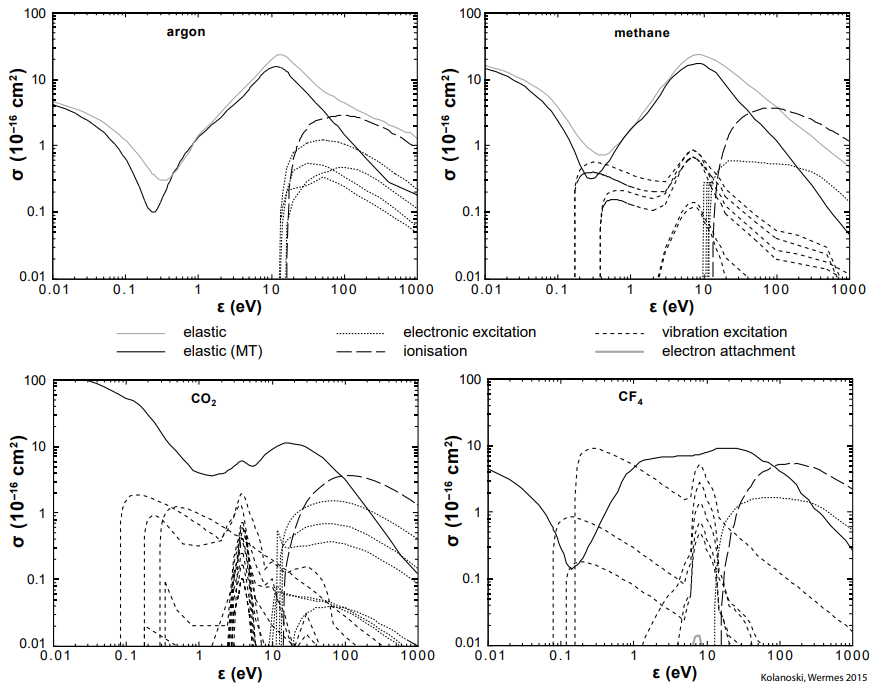
\includegraphics[width=0.95\textwidth,frame]{Chapters/images/Interazione_radiazione_materia/image-20220222172045918.png}

  \end{figure}

  \begin{figure}[H]
    \centering
    \captionsetup{width=0.95\linewidth}
    \caption{Sezioni d'urto in funzione dell'energia.\\ Si noti che per molecole semplici si ha per lo più solo scattering elastico.\\ Nelle regioni di scattering elastico la mobilità cresce molto all'aumentare dell'energia}
    \label{fig:gascross}
  \end{figure}




 \vspace{-20pt}
  \begin{remark}[Mistura argon metano]  \hfill \\ 
\hspace{-50pt}
  \begin{minipage}{0.32\textwidth}
    \begin{figure}[H]
        \centering
        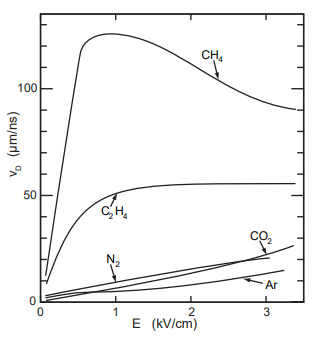
\includegraphics[height=4.8cm,frame]{Chapters/images/Interazione_radiazione_materia/image-20220222172819847.png}
    \end{figure}
  \end{minipage} \hspace{-10pt}
  \begin{minipage}{0.64\textwidth}
  \begin{figure}[H]
    \centering
    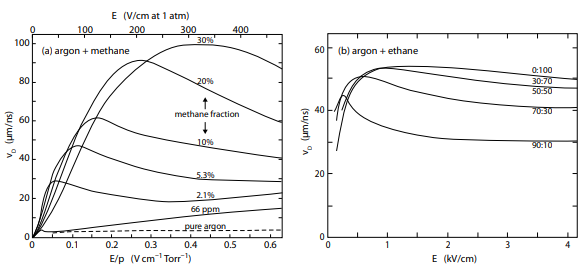
\includegraphics[height=4.8cm,frame]{Chapters/images/Interazione_radiazione_materia/image-20220222172607946.png}
  \end{figure}

  \end{minipage}
\begin{figure}[H]
    \captionsetup{width=\textwidth}
    \caption{Andamento della velocità di drift in funzione del campo elettrico per diversi materiali.}
    Aggiungere metano all' argon causa una diminuzione nella distribuzione di energia degli elettroni quindi le sezioni d'urto diminuiscono e la velocità di drift aumenta.\\ 
    Infatti tipicamente viene aggiunto metano all'argon.
\end{figure}

  \end{remark}
\subsection*{Diffusione}
Nei gas si è spesso al di fuori del limite termico e la dispersione è un problema serio che va moderato

\hspace{-25pt}
\begin{minipage}{0.7\textwidth}
    \begin{figure}[H]
        \centering
        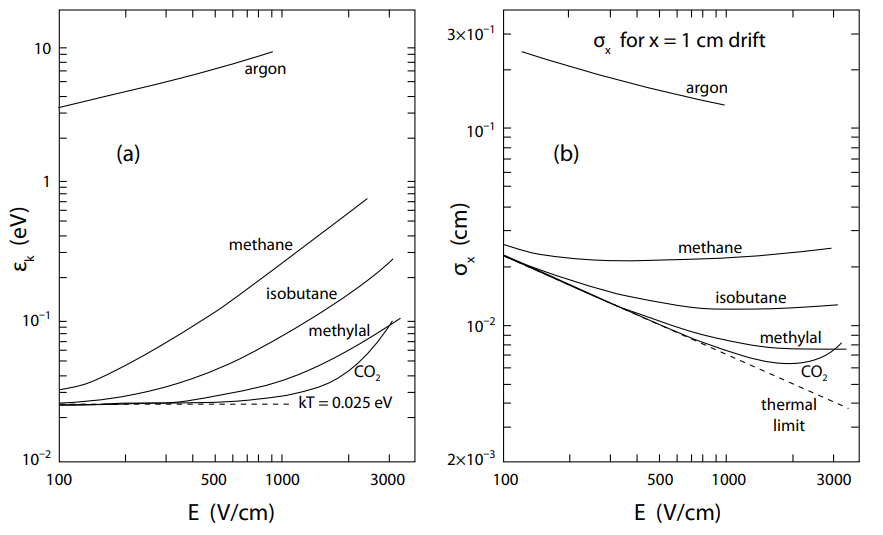
\includegraphics[width=\textwidth,frame]{Chapters/images/Interazione_radiazione_materia/image-20220222180147403.png}
    \end{figure}
\end{minipage}
\begin{minipage}{0.35\textwidth}
\begin{figure}[H]
    \centering
    \captionsetup{width=\textwidth}
    \caption{A: Energia caratteristica per diversi gas in funzione del campo elettrico. (Il limite termico si ha per campo elettrico nullo)
    \\ B: Dispersione per centimetro percorso in vari gas.\\ Si noti come una carica dell'argon, dopo aver percorso 1cm, ha già 1mm di dispersione circa}
\end{figure}
\end{minipage}

\hspace{-25pt}
\begin{minipage}{0.35\textwidth}
    \begin{figure}[H]
        \centering
        \captionsetup{width=\textwidth}
        \caption{La dispersione non è isotropa e spesso bisogna tenere conto delle differenze tra quelle longitudinali e quelle trasversali (quindi abbiamo due coefficienti di dispersione $D_T$ e $D_L$)\\ Addirittura in presenza di campo B l'anisotropia è così forte che D va scritto in forma tensoriale}
    \end{figure}
\end{minipage} \hfill
\begin{minipage}{0.7\textwidth}

    \begin{figure}[H]
        \centering
        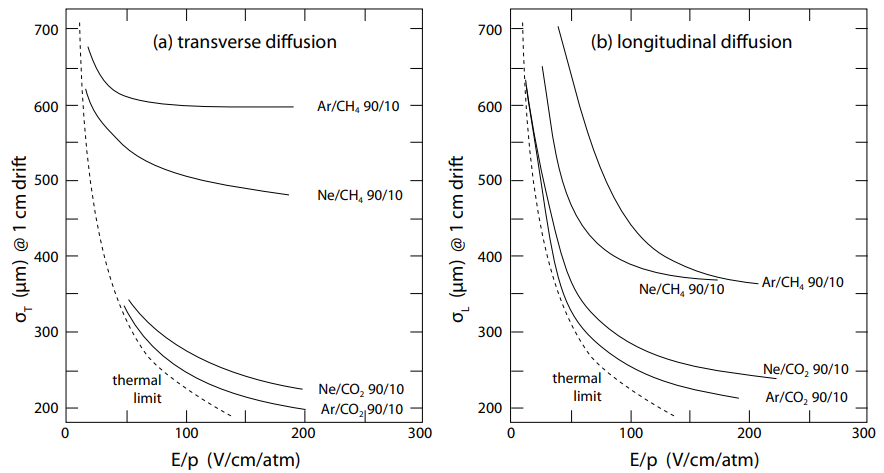
\includegraphics[width=\textwidth,frame]{Chapters/images/Interazione_radiazione_materia/image-20220222180339979.png}
        \captionsetup{width=\textwidth}
    \end{figure}
\end{minipage}

\newpage
\section{Moto delle cariche nei semiconduttori}
La massa (effettiva) delle lacune non è perfettamente definita ma p comparabile a quella degli elettroni quindi il comportamento delle cariche positive è totalmente diverso da quello degli ioni nei gas.

\subsection*{Velocità di Drift}
Lo scattering nel reticolo, prevalentemente dovuto alle impurità, è molto diverso reispetto a quello nei gas (quindi cambia l'integrale di collisione) e le perdite di energia in fononi  può essere molto rilevante

\hspace{-30pt}
\begin{minipage}{0.55\textwidth}
    \vspace{-40pt}
    \begin{figure}[H]
        \centering
        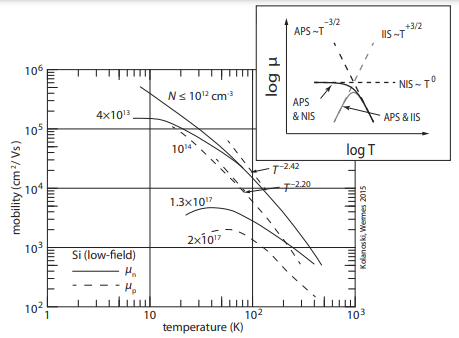
\includegraphics[width=\textwidth,frame]{Chapters/images/Interazione_radiazione_materia/image-20220223184712151.png}
        \captionsetup{width=\textwidth}
        \caption{Mobilità in funzione della temperatura per diverse densità di doping. \\ Nel caso di temperature moltobasse la mobilità è molto alta, per questo motivo si costruiscono rivelatori criogenici.\\ Nota che la curva APS significa "acustic phono scattering"}
        \label{fig:}
    \end{figure}
\end{minipage} \hspace{5pt}
\begin{minipage}{0.5\textwidth}

    Anche qui è presente un effetto di \textbf{saturazione} : la velocità di drift cresce con il campo elettrico fino ad arrivare a una saturazione e, in alcuni casi, anche a una diminuzione per campi elettrici molto alti (a causa di scattering inelastici con fononi di più alta energia).\\ 
    Una buona descrizione della velocità di drift può essere data da:
    $$
    v_d=\mu(E) E =\frac{\mu_0 E}{[1+(\frac{\mu_0 E}{v_{\text{sat}}})^\beta]^{^{1/\beta}}}
    $$
    dove $\mu_0$ è la mobilità a basso campo, $v_{\text{sat}}$ è la velocità di saturazione e $\beta$ è un parametro empirico (genericamente diverso per elettroni e lacune) con un valore tra 1 e 2.\\
    Ad esempio per il \textbf{silicio} (fattore 3): \[\begin{gathered}
        \mu_n=1450 cm^2/(Vs) \; \\  \; \mu_p=500 cm^2/(Vs)
    \end{gathered}\] 
\\ \\ 
\end{minipage}
\vspace{-40pt}\par\noindent\hspace*{0pt}\ignorespaces
Nei gas la mobilità era dell'ordine di $10 cm^2/\text{Vs} $ per gli ioni e $10^4 cm^2/\text{Vs} $ per gli $e^{-}$ 

\hspace{-20pt} 
\begin{minipage}{0.55\textwidth}
    \vspace{-5pt}
    \begin{figure}[H]
        \centering
        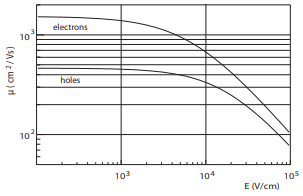
\includegraphics[width=\textwidth,frame]{Chapters/images/Interazione_radiazione_materia/image-20220223185948941.png}

        \label{fig:mobilitae}
    \end{figure}
\end{minipage} \hspace{5pt}
\begin{minipage}{0.48\textwidth}
\begin{figure}[H]
    \centering
    \captionsetup{width=\textwidth}
    \vspace{-10pt}
    \caption{Mobilità di elettroni e cariche in funzione del campo elettrico nel silicio a temperatura ambiente}
\end{figure}
\vspace{-30pt}
    \begin{note}Nei semiconduttori è possibile arrivare a campi elettrici molto maggiori visto che le differenze di potenziale sono applicate su scale molto più piccole (microscopiche), quindi non c'è bisogno di arrivare a voltaggi esagerati come nei rivelatori a gas
    
    \end{note}

\end{minipage}

\begin{figure}[H]
    \centering
    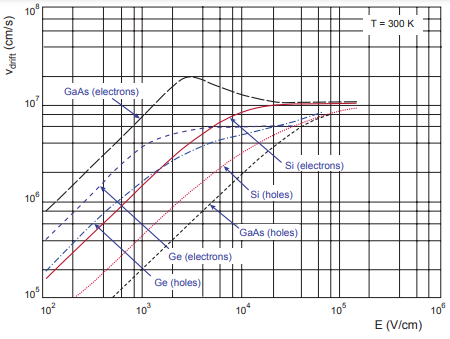
\includegraphics[width=0.9\textwidth,frame]{Chapters/images/Interazione_radiazione_materia/image-20220223190024373.png}
    \captionsetup{width=0.9\textwidth}
    \caption{Velocità di drift in funzione del campo elettrico. Si noti che prima della saturazione la velocità di drift è proporzionale al campo (slope $\simeq1$)}
    \label{fig:driftvel}
\end{figure}
\subsection*{Diffusione}
Come nel caso degli ioni nei gas, nei semiconduttori si è vicini al limite termico quindi vale approssimativamente $\epsilon_k=qD/\mu=kT$ (ovviamente si ha un D e un $\mu$ diverso per elettroni e lacune)

\section{Formazione del segnale (Schokley-Ramo)}
Quando la carica si avvicina a un elettrodo su esso viene indotta una carica del segno opposto . Mettendo l'elettrodo a possiamo far fluire una corrente
\begin{note}non è la collezione della carica a formare il segnale ma la carica indotta. Quando la caricha prodotta dalla ionizzazione viene collezionata dall'elettrodo  il segnale cessa di esistere

\end{note}

\subsection{Wighting field}
Consideriamo una carica q che si muove in un sistema di 2 elettrodi
\begin{figure}[H]
    \centering
    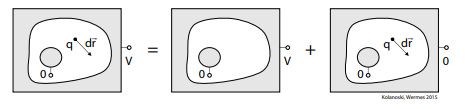
\includegraphics[width=0.7\textwidth,frame]{Chapters/images/Interazione_radiazione_materia/image-20220223201749719.png}
    \captionsetup{width=0.7\textwidth}
\end{figure}
La differenza di potenziale tra i due elettrodi induce una carica Q e -Q su di essi. Data la capacità del sistema si ha $Q=CV$.
\begin{itemize}
    \item Una carica in moto tra gli elettrodi induce una carica addizionale e il campo elettrico fa un lavoro $ dW_q=q \vec{E_0} d\vec{r} $

\begin{remark}\hfill \\ 
    Dal lavoro del campo la carica acquista energia cinetica che viene dissipata nelle collisioni. In questo caso è rilevante solo l'energia che il campo elettrico degli elettrodi fornisce a prescindere dalla dissipazione di energia della carica
\end{remark}

\item Questo lavoro deve essere fornito o dal campo ($dW_E$) o dalla sorgente ($dW_V=dQ\: V +Q dV=dQ\: V$ poiche V costante).
  Per conservazione dell'energia vale

$$
dW_E+dW_V+dW_q=0
$$

> Convenzione: dQ negativa se una carica negativa e spostata nella sorgente (o se una carica positiva è rimossa dalla sorgente)

\item L'energia del campo nel volume $\tau$ è $W_E=\frac{1}{2}\epsilon \epsilon_0 \int_\tau \vec{E}^2 d\tau$

\item Sfuttando il principio di sovrapposizione scriviamo il campo come somma di quello generato dal passaggio della carica e quello degli elettrodi $\vec{E}=\vec{E_0}+\vec{E_q}$

\item Il lavoro sulla carica q verrà fatto da $E_0$ (come scritto sopra) mentre $E_q$ non contribuisce al lavoro

\item Sfruttiamo il principio di sovrapposizione anche con i potenziali $\phi=\phi_0+\phi_q$ . Per $\phi_0$ le condizioni al contorno sono date dai valori di potenziale sugli elettrodi mentre per $\phi_q$ vale $\phi_q|_\partial=0$

\item Le equazioni di Poisson/Laplace saranno
  $$
  \nabla^2\phi_0=0
  \\
  \nabla^2\phi_q=-\frac{q}{\epsilon \epsilon_0}\delta(\vec{r}-\vec{r_q})
  \\
  \vec{E_i}=-\vec{\nabla}\phi_i
  $$

\item Anche il lavoro è separabile in due componenti (per il teorema di Green) $dW_E=dW_{E_q}+dW_{E_0}$.
  Se assumiamo che il campo $E_0$ è statico e che $E_q$ non fa lavoro (nemmeno scambiando energia con la sorgente che è a V costante) allora vale $dW_E=0$

\item Quindi si ha
  $$
  dW_q+dW_V=q\vec{E_0} d\vec{r}+dQ \: V=0 \implies 
  \\
  \implies dQ \: V = -q\vec{E_0} d\vec{r}
  $$
  Che significa che il lavoro sulla carica q è fornito dalla sorgente 

\item Il campo $E_0$ dipende dalla geometria ma il suo valore assoluto dipende da proporzionalmente da V, quindi il rapporto $E_0/V$ è indipendente da V.

\item Per semplicità poniamo V=1 e definiamo i campi/potenziali di weighting come $\phi_w=\phi_0/V$ e $\vec{E_w}=-\vec{\nabla}\phi_w$. (potenziale di weighting è privo di dimensioni e il campo è l'inverso di una lunghezza)

\item La carica che genera il segnale è $dQ=-q\vec{E_w}d\vec{r}$

\item Poichè $d\vec{r}/dt=\vec{v_D}$ (velocità di drift) possiamo esprimere la corrente come
  $$
  i_s=-\frac{dQ}{dt}=q\vec{E_w}\vec{v_D}
  $$
  In generale la direzione della velocità di drift può essere diversa da quella del campo di weighting

\begin{note}[Approssimazione]\hfill \\ 
    abbiamo ignorato la presenza di campi magnetici, cariche di polarizzazione o di altre densità di cariche all'interno del volume
\end{note}

\end{itemize}

\subsection{Teorema di Shockley-Ramo}

Consideriamo un arrangiamento di k elettrodi con potenziali $V_1,... , V_k$
\begin{itemize}
    \item Per sovrapposizione $\phi_0 = \sum_i^k\phi_i$ con $\phi_i=V_i$ sull'elettrodo i-esimo e 0 altrove
\item Definiamo il potenziale di weighting come $\phi_{w,i}=\phi_i/V_i$, ognuno di questi risolve l'eq. di Laplace
\item Generalizzando quanto visto sopra si ha $i_{S,i}=q\vec{E}_{w,i}\vec{v}_D$
\end{itemize}




\begin{remark}
\begin{itemize}
    \item La velocità di drift dipende dal campo elettrico dotale (comprese le polarizzazioni dei materiali) $\vec{v}_D=\mu \vec{E}$
    \item Il weighting field rappresenta l'accoppiamento di un punto da ogni elettrodo calcolato dall'eq. di Laplace
    \item Se la carica viene prodotta molto vicino a un elettrodo il segnale su quello non sarà vista e allo stesso modo la carica indotta sarà quasi nulla
    \item La mobilità domina quindi normalmente domina il segnale degli elettrondi ma sa è presente moltiplicazione nei pressi dell'anodo domina il segnale degli ioni che devono attraversare tutto il detector per arrivare al catodo
\end{itemize}
\end{remark}

\subsection{Esempi}
\sssec{Camere a ionizzazione}
Consideriamo due elettrodi a distanza d siemipi da del gas e una carica che viene prodotta per ionizzazione a distanza $x_0$ da un elettrodo
\begin{figure}[H]
    \centering
    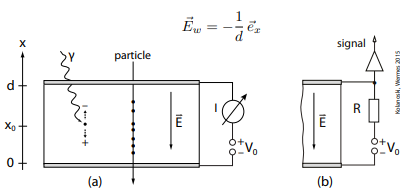
\includegraphics[width=0.7\textwidth,frame]{Chapters/images/Interazione_radiazione_materia/image-20220223210231074.png}
\end{figure}
Il campo è $E=-\frac{V}{d} \;\hat{x}$ quindi il campo di weighting è $E_w=-\frac{1}{d}\hat{x}$ e quindi la corrente generata da elettroni e ioni è

\[
    \begin{gathered}
        i_s^\pm=-\frac{q^\pm}{d}\vec{v}_D^\pm \; \hat{x}
        \\ 
        T^-=\frac{d-x_0}{{v}_D^-} \; ; \; T^+=\frac{x_0}{{v}_D^+}
    \end{gathered}
\]
dove $T^\pm$ sono le durate dei due segnali (ovvero il tempo che le cariche ci mettono ad arrivare agli elettrodi)


\begin{minipage}{0.48\textwidth}
    \vspace{-2pt}
    \begin{figure}[H]
        \centering
        \captionsetup{width=\textwidth}
        \caption{Segnale della corrente misurata agli elettrodi.\\ In questo caso il rapporto tra le velocità di drift è posto a 1/3 ma tipicamente è 1/1000}
        \vspace{-7pt}
        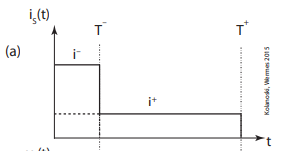
\includegraphics[width=\textwidth,frame]{Chapters/images/Interazione_radiazione_materia/image-20220223211327802.png}

        \label{fig:}
    \end{figure}
    \vspace{-30pt}
    \begin{figure}[H]
        \centering
        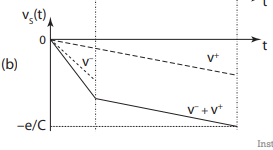
\includegraphics[width=\textwidth,frame]{Chapters/images/Interazione_radiazione_materia/image-20220223212101007.png}
        \captionsetup{width=\textwidth}
        \vspace{-23pt}
        \caption{Si può anche misurare il voltaggio invece della corrente.\\ 
        Per farlo basta inserire in una resistenza con la ionization chamber che fa da condensatore. Il tempo RC  del circuito deve essere maggiore del tempo di drift}
        \label{fig:}
    \end{figure}
\end{minipage} \hfill
\begin{minipage}{0.48\textwidth}
    \vspace{3pt}
    \begin{figure}[H]
        \centering
        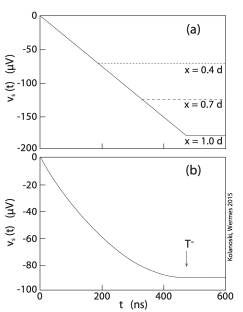
\includegraphics[width=\textwidth,frame]{Chapters/images/Interazione_radiazione_materia/image-20220223212235264.png}
        \captionsetup{width=\textwidth}
        \vspace{-19pt}
        \caption{Se invece di avere una signola carica prodotta abbiamo una linea lungo il quale vengono prodotte le cariche (traccia della particella) bisogna sommare i diversi contributi\\ A: Voltaggi misurati per singola carica prodotta\\ B: Somma dei contributi per una line di cariche}
        \label{fig:}
    \end{figure}

\end{minipage}
\sssec{Contatori proporzionali}
\begin{figure}[H]
    \centering
    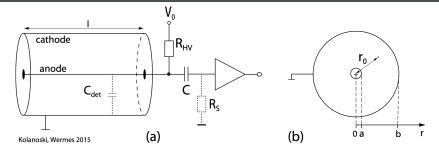
\includegraphics[width=0.7\textwidth,frame]{Chapters/images/Interazione_radiazione_materia/image-20220223212504142.png}

\end{figure}
In simmetria cilindrica il campo di weighting è $\vec{E}_w=\frac{1}{r}\frac{1}{\ln(b/a)} \; \hat{r}$ dove b e a dono il raggio di anodo e catodo
\\ 
Dalla dipendenza $1/r$ ne consegue che il segnale è dominato dal modo vicino all'anodo.
Vicino all'anodo avviene moltiplicazione di carica per un fattore $10^3-10^6$. 
\\ 
Questo significa che il segnale è dominato dal moto degli ioni prodotti dalla moltiplicazione che attraversano tutta la distanza che va dall'anodo al catodo
\begin{figure}[H]
    \centering
    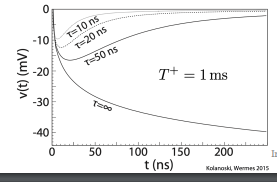
\includegraphics[width=0.5\textwidth,frame]{Chapters/images/Interazione_radiazione_materia/image-20220223213221551.png}
    \captionsetup{width=0.5\textwidth}
    \caption{La forma del segnale è principalmene stabilita dal circuito di lettura e del suo tempo caratteristico}
\end{figure}

\sssec{Detector a semiconduttore}

\begin{figure}[H]
    \centering
    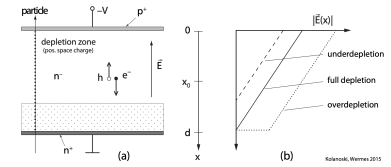
\includegraphics[width=0.7\textwidth,frame]{Chapters/images/Interazione_radiazione_materia/image-20220223213733948.png}
    \captionsetup{width=0.9\textwidth}
    \caption{Nei semiconduttori il campo elettrico non è costante a causa della presenza di molte cariche spaziali (soprattutto nella depleted zone)}
\end{figure}

\begin{figure}[H]
    \centering
    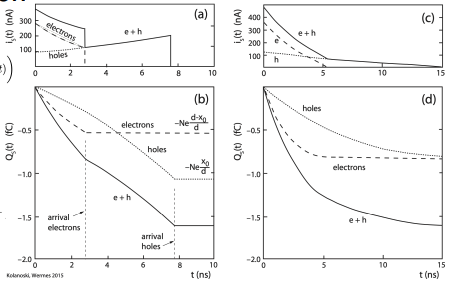
\includegraphics[width=0.7\textwidth,frame]{Chapters/images/Interazione_radiazione_materia/image-20220223213850670.png}
    \captionsetup{width=0.7\textwidth}
    \captionsetup{width=0.9\textwidth}
    \caption{Quindi in questo caso la forma dei segnali è molto più complicata ma sono essenzialmente sezioni di esponenziale (poichè il campo elettrico è lineare in funzione della posizione nella depletion zone)}
    \label{fig:}
\end{figure}

\begin{remark}[Elettrodi segmentati] \hfill \\ 
    Quando si hanno elettrodi segmentati (es. delle strip) anche se la carica verrà collezionata da un elettrodo anche gli altri vicini vedranno un segnale a causa del moto della carica
    \begin{figure}[H]
        \centering
        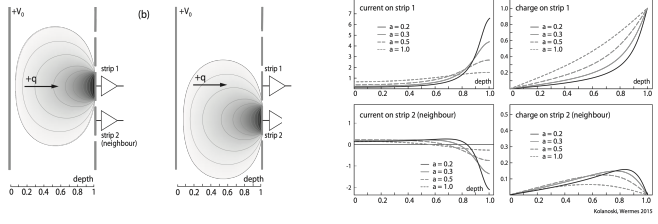
\includegraphics[width=0.7\textwidth,frame]{Chapters/images/Interazione_radiazione_materia/image-20220223214312686.png}
    \end{figure}
    Sulla strip 2 la corrente è negativa perchè vicino alla strip il campo di weighting cambia segno
\end{remark}

\section{Rumore}\footnote{Questa parte (sul rumore) l'ho tirata via molto a caso. Se vuoi qualcosa di più preciso vai a riprendere gli appunti sull'analisi dati delle onde gravitazionali}
\begin{figure}[H]
    \centering
    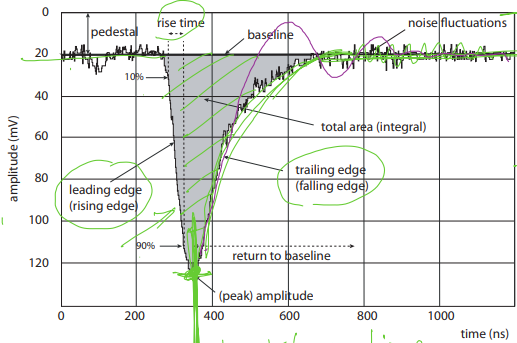
\includegraphics[width=0.7\textwidth,frame]{Chapters/images/Interazione_radiazione_materia/image-20220223230311045.png}
    \captionsetup{width=0.7\textwidth}
    \caption{Tipico segnale osservato in uscita di un detector.\\ Il tempo di rise dipende principalmente dalle caratteristiche del rivelatore ma quello di rilassamento principalmente dall'elettronica.\\ Volendo si può studiare anche la carica accumulata considerando l'area del segnale}
\end{figure}

\begin{definition*}
    \textbf{undershoot}: Quando si hanno segnali molto veloci in risalit il segnale può avere un picco che va sopra lo 0. 
In questo caso non si può usare l'area del segnale per studiare la carica collezionata

\end{definition*}

\begin{figure}[H]
    \centering
    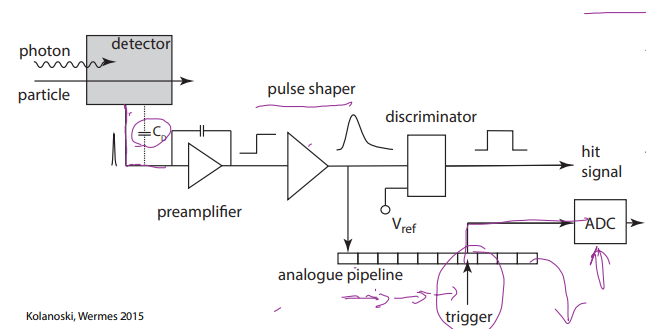
\includegraphics[width=0.7\textwidth,frame]{Chapters/images/Interazione_radiazione_materia/image-20220223230709058.png}
    \captionsetup{width=0.7\textwidth}
    \caption{Tipica catena di lettura}
\end{figure}
Per lo studio del rumore facciamo un \textbf{assunzione di ergodicità} ovvero che $<g(x)>=lim_{T\to \infty} \int_0^T g(x(t))dt$. In questo modo possiamo usare le misure fatte su $x(t)$

Alcune quantità e relazioni importanti sono:
\begin{itemize}
    \item \textbf{Autocorrelazione}  $\phi(\tau)=\overline{X(t)X(t+\tau)}$:
    \begin{itemize}
        \item E' indipendente da t poichè consideriamo il processo stazionario
        \item $\phi(0)=Var(X)$
        \item Se $\phi(\tau)\propto \delta(\tau)$ siamo in presenza di \textbf{rumore bianco}
    \end{itemize}
    \item \textbf{Densità spettrale} $S_x(f)=lim_{T\to \infty}2T\; \overline{a_na_n^*}|_{n=fT}$ dove gli $a_n $ sono i coefficienti della serie di Fourier.
    \begin{itemize}
        \item Questa quantità è legata alla varianza del segnale per unità di frequenza. Più precisamente vale $S_x(f)df=\overline{x_n^2}$ (che è la varianza se segnale  stazionario a media nulla)

\item Legata alla funzione di autocorrelazione tramite una trasformata di Fourier

\item Dimensioni: $V^2/Hz$ oppure $A^2/Hz$

\item Spesso si usa la sua radice (ovvero la amplitude spectral density)

\item Dato un segnale in input X, una funzione di trasferimento g(f) e un segnale di output Y vale:
  $S_Y(f)=|g(f)|^2 S_X(f)$ .

  Per misurare $S_X$ in genere si usa un amplificatore molto piccato intorno una frequenza $f_0$ e s i usa approssimazione $$\begin{gathered}
      \overline{Y^2}=\int_0^\infty |g(f)|^2 S_X(f)df\sim S_X(f_0)|g(f_0)|^2\int_0^\infty |\frac{g(f)}{g(f_0)}|^2  \implies \\  \implies S_X(f_0)=\frac{\overline{Y^2}}{g(f_0)^2B_N}
  \end{gathered}$$ dove $B_N$ è l'ultimo integrale rimanente sopra e viene chiamato \textit{gain bandwidth product}
    \end{itemize}
\end{itemize}

\subsection{Sorgenti di rumore}
\begin{itemize}
    \item \textbf{Rumore termico (Jhonson)}: Dovuto all'agitazione termica delle cariche ai capi di una resistenza

    E' un rumore bianco con PSD $S_V(f)=4kTR$ dove R è la resistenza (o se misuriamo la corrente $S_I=4kT/R$ poichè $I^2=V^2/R^2$)
  
  \item \textbf{Shot noise}: fluttuazione poissoniana del numero di portatori di carica $S_I=2\overline{I}e$
    (La dim. si effettua semplicemente facendo il calcolo della PSD partendo da un segnale $\overline{I(t)}=\sum_i e\delta(t-t_i)$)
  
   \begin{note}
    sia il rumore termico che lo shot noise sono rumore bianco
   \end{note} 
  
  \item \textbf{Rumore 1/f}: Rumore non ancora ben compreso dovuto a fenomeni di interfaccia. Empiricamente ha PSD $S_V=A/f^\alpha$ con $\alpha \sim 0.8-1.5$ e A costante
  
  \item Le varie PDS dovute ai diversi tipi di rumore vanno somate in quadratura
  
  Le sorgenti di rumore possono essere:
  
  \item \textbf{Detector}: a causa di rumori termici, correnti di age e fenomeni induttivi e autoinduttivi
  \item \textbf{Elettronica}: Rumore intrinsico dei componenti attivi, capacità in input (compreso il detector), altri fenomeni induttivi e autoinduttivi
  \item \textbf{Trasmissione}: Resistenza, capacità e induttanza/autoinduttanza dei cavi
  
  E' molto importante mantenere alto il \textbf{rapporto segnale rumore (SNR)}.
  Il rumore effettivo del sistema dipende dalle proprietà di filtraggio dell'amplificatore e la capacità in input gioca un ruolo fondamentale (grandi capacità causano rumori maggiori).
  
  Per tenere sotto controllo rumore termico e quello shot bisogna mantenere correnti basse, temperature basse e bandwidth strette.
  Il rumore 1/f invece dipende dal processo di fabbricaazione.
  
  Anche la massa gioca un ruolo fondamentale, tutte le masse devono finire nello stesso identico pozzo
\end{itemize}

\begin{eg}[Misuramento di carica] \hfill \\ 
    In un sistema simile si vuole massimizzare il rapporto segnale rumore inteso come carica/deviazione standard del segnale (detto anche ENC)
Considerando tutti gli errori e sommandoli in quadratura 

\begin{figure}[H]
    \centering
    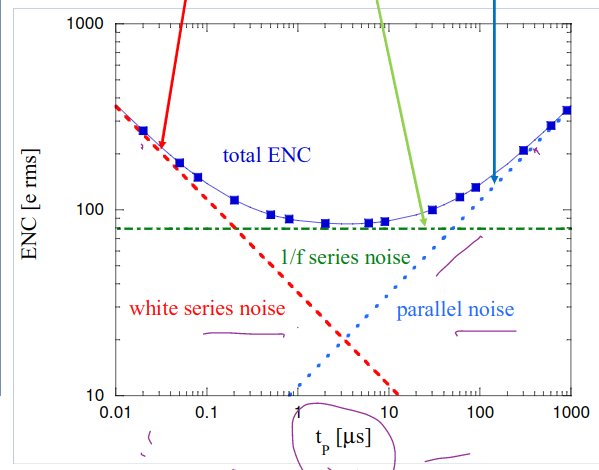
\includegraphics[width=0.7\textwidth,frame]{Chapters/images/Interazione_radiazione_materia/image-20220302174553973.png}
    \captionsetup{width=0.7\textwidth}
    \caption{$t_p$ è il tempo di picco ovvero il tempo necessario a raggiungere il picco del segnale)}

\end{figure}
si nota come bisogna scegliere un tradeoff tra diverse situazioni
\end{eg}